\documentclass{beamer}
\usepackage{wrapfig}
\usepackage{tikz}
\usepackage{tkz-berge} 
\usepackage{verbatim}
\usepackage{algorithm,algorithmic}
\mode<presentation>

{
  \usetheme{Warsaw}

 \setbeamertemplate{footline}{}
\setbeamercovered{transparent}
\usepackage{color}
\title{A programming approach to vertex coloring by kernelization}
\author{{Mehri Bagherihamaneh}\\[1cm]{\small {Advisor: Prof. Dr. Arie M.C.A. Koster}}\\[.5cm]{\small {Lehr-und Forschungsgebiet Diskrete Optimierung}}\\ {\small {Rheinisch-Westfaelische Technische Hochschule Aachen}}}

{\small \date{{Aachen, }\today}}


\begin{document}

\begin{frame}
  \titlepage
\end{frame}


\begin{frame}{What this thesis is about?}
\begin{itemize}

\item Graph vertex coloring

\item Using kernelization to solve vertex coloring with reduction of size of the  graph
\item Demonstrate kernelization in some sample graphs in practice
\item "improved DSATUR-based Branch and Bound" algorithm
\item Python is used as programming language

\end{itemize}
\end{frame}

\begin{frame}{Introduction}


\begin{enumerate}
\item Some definitions
\item Special kernelization for vertex coloring

\item Min vertex cover
\item An example

\item An exact algorithm for vertex coloring

\item Computational experiments
\item conclusion
\end{enumerate}
\end{frame}



\begin{frame}{Definitions-Vertex coloring}


\begin{definition}
A \color{red} vertex coloring \color{black} is an assignment of colors to each vertex of a graph such that no edge connects two vertices with the same  color.
\end{definition}
\begin{definition}
The \color{red} chromatic number \color{black} of a graph is the smallest number of colors needed for vertex coloring and denoted by $\chi(G)$. 
\end{definition}
\begin{definition}
A \color{red} proper $k$-coloring \color{black} is an assignment of $k$ colors to the vertices of a graph so that no two adjacent vertices have the same color: $f: V(G) \to \{1, 2, 3, . . . , k\}$, for all edges $\{u, v\}$ we have $f(u) \not= f(v)$.
\end{definition}
\end{frame}


\begin{frame}{Example-Vertex coloring}
\begin{example}
The petersen graph is $3$-colorable:

\begin{center}
\begin{tikzpicture}[rotate=90]
  \GraphInit[vstyle=Hasse]
  \SetVertexNoLabel \SetUpVertex[MinSize=2pt] \grPetersen[RA=2,RB=1]
  \SetUpVertex[inner sep=1pt,MinSize=2pt]
  \AddVertexColor{red}{a0,b1,b2,a3}
  \AddVertexColor{green}{a1,b0,a4}
  \AddVertexColor{blue}{b4,b3,a2}
\end{tikzpicture}
\end{center}
\end{example}
\end{frame}

\begin{frame}{Definitions-Vertex cover}
\begin{definition}
A \color{red} vertex cover \color{black} $V'$ of a graph is a subset of $V$ such that for every edge $uv \in E$ , $u \in V'$ or $v \in V'$ , that means every edge has at least one endpoint in the vertex cover. 
\end{definition}
\begin{definition}
The \color{red} minimum vertex cover \color{black} problem is the problem of finding a vertex  cover with minimum number of vertices in a given graph. The size of minimum vertex cover is called the vertex cover number and denoted by $\tau(G)$ .
\end{definition}
\end{frame}

\begin{frame}{Example-Vertex cover}
\begin{example}
Vertex cover:
\begin{center}
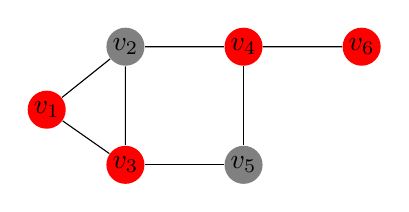
\begin{tikzpicture}
\node[circle,fill=red,inner sep=1pt,minimum size=1mm] (v1) at (0,0.2) {$v_1$};
\node[circle,fill=gray,inner sep=1pt,minimum size=1mm] (v2) at (1,1) {$v_2$};
\node[circle,fill=red,inner sep=1pt,minimum size=1mm] (v3) at (1,-0.5) {$v_3$};
\node[circle,fill=red,inner sep=1pt,minimum size=1mm] (v4) at (2.5,1) {$v_4$};
\node[circle,fill=gray,inner sep=1pt,minimum size=1mm] (v5) at (2.5,-0.5) {$v_5$};
\node[circle,fill=red,inner sep=1pt,minimum size=1mm] (v6) at (4,1) {$v_6$};

\draw (v1)--(v2)--(v4)--(v6);
\draw (v1)--(v3)--(v2);
\draw (v3)--(v5)--(v4);
\end{tikzpicture}

\end{center}


Min vertex cover:
\begin{center}
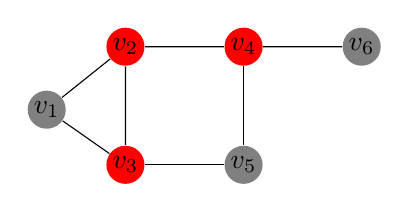
\begin{tikzpicture}
\node[circle,fill=gray,inner sep=1pt,minimum size=1mm] (v1) at (7,0.2) {$v_1$};
\node[circle,fill=red,inner sep=1pt,minimum size=1mm] (v2) at (8,1) {$v_2$};
\node[circle,fill=red,inner sep=1pt,minimum size=1mm] (v3) at (8,-0.5) {$v_3$};
\node[circle,fill=red,inner sep=1pt,minimum size=1mm] (v4) at (9.5,1) {$v_4$};
\node[circle,fill=gray,inner sep=1pt,minimum size=1mm] (v5) at (9.5,-0.5) {$v_5$};
\node[circle,fill=gray,inner sep=1pt,minimum size=1mm] (v6) at (11,1) {$v_6$};

\draw (v1)--(v2)--(v4)--(v6);
\draw (v1)--(v3)--(v2);
\draw (v3)--(v5)--(v4);
\end{tikzpicture}
\end{center}
\end{example}
\end{frame}

\begin{frame}{Definitions-Clique}
\begin{definition}
A \color{red} clique \color{black} in a graph is a subset of vertices such that every two distinct vertices are adjacent. 

A \color{red} maximal clique \color{black} is a clique that cannot be extended by adding one more adjacent vertex. 
\end{definition}
\begin{definition}
A \color{red} maximum clique \color{black} is a clique that has the maximum possible number of vertices. The clique number, $\omega(G)$, is the number of vertices in a maximum clique of $G$. 
\end{definition}

\end{frame}

\begin{frame}{Example-Clique}
\begin{example}
\begin{center}
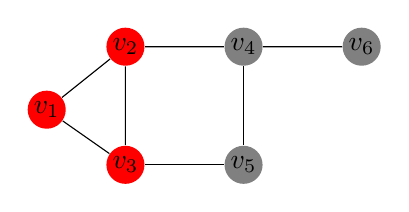
\begin{tikzpicture}
\node[circle,fill=red,inner sep=1pt,minimum size=1mm] (v1) at (0,0.2) {$v_1$};
\node[circle,fill=red,inner sep=1pt,minimum size=1mm] (v2) at (1,1) {$v_2$};
\node[circle,fill=red,inner sep=1pt,minimum size=1mm] (v3) at (1,-0.5) {$v_3$};
\node[circle,fill=gray,inner sep=1pt,minimum size=1mm] (v4) at (2.5,1) {$v_4$};
\node[circle,fill=gray,inner sep=1pt,minimum size=1mm] (v5) at (2.5,-0.5) {$v_5$};
\node[circle,fill=gray,inner sep=1pt,minimum size=1mm] (v6) at (4,1) {$v_6$};

\draw (v1)--(v2)--(v4)--(v6);
\draw (v1)--(v3)--(v2);
\draw (v3)--(v5)--(v4);
\end{tikzpicture}
\end{center}
\end{example}
\end{frame}


\begin{comment}
\begin{frame}{Propositional logic}
\begin{definition}
A propositional logic formula is constructed by some variables using operators AND ("$\land$"), OR ("$\lor$"), NOT ("$\lnot$") and parentheses. 

A clause is an expression constructed from a finite  disjunction or conjunction of literals.
\end{definition}



\begin{definition}
A boolean formula is satisfiable if it can be TRUE by assigning logical values to its variables. 
\end{definition}
\end{frame}
\begin{frame}{Propositional logic}


\begin{example}

\item $x_1 \land (x_2 \lor\lnot x_1)$, where $(x_2 \lor\lnot x_1)$ is a clause.

\end{example}
\begin{example}
 $\varphi = d\lor (a\land b\land (c\lor d \land\lnot a))$

\begin{table}[H]
\begin{center}
\begin{tabular}{c|c|c|c|c}
$a$ & $b$ & $c$ & $d$ & $\varphi$\\
\hline
F & F & F & T & T\\ 
&&&&\\
&&&&\\
\end{tabular}
\end{center}
\end{table}
\end{example}

\begin{example}
Unsatisfiable formula:

\begin{center}
$\theta = X \land \lnot X$
\end{center}
\end{example}

\end{frame}

\begin{frame}{Propositional logic}
\begin{definition}
A boolean formula is in conjunctive normal form (CNF) if it is a conjunction of one or more disjunctions of variables.
\end{definition}

\begin{example}
\item $\lnot x \land (y \lor z)$
\end{example}

\begin{definition}
For a given CNF formula $\varphi$, the boolean satisfiability problem (SAT) is a decision problem which asks whether the formula $\varphi$ is satisfiable. The $3$-SAT problem is a SAT problem with at most $3$ variables in each clause. 
\end{definition}

\begin{theorem}
The $3$-SAT problem is $NP$-complete.
\end{theorem}
\end{frame}


\begin{frame}{Complexity}
\begin{definition}
For an instance $I$ from instance set $\mathcal{I}$, a decision problem $\Pi$ is a YES-NO question which asks if
there is at least one solution for the problem $\Pi$ in $I$.
\end{definition}
\begin{example}
$k$-COLORING is a decision problem, which asks if we can color a graph $G$ with $k\in\mathbb{N}$ or fewer colors. For $k \geq 3$ in general graphs, $k$-COLORING is $NP$-complete.
\end{example}
\end{frame}


\begin{frame}{Complexity}
\begin{itemize}
\item class $P$ (PTIME)

\color{green} Example: \color{black} the problem of determining if a number is prime.

\item $NP$ (non-deterministic polynomial) $P\subset NP$.

\item $NP$-hard class 

\color{green} Example: \color{black} traveling salesman problem.

If $P \not= NP$, $NP$-hard problems cannot be solved in polynomial time. 

\item $NP$-complete class:  $L$ is $NP$-complete if:
\begin{enumerate}
\item $L$ is $NP$-hard.

\item $L$ is in $NP$.
\end{enumerate}
\end{itemize}
\end{frame}


\begin{frame}{Is $P = NP$ or $P \not= NP$?}

%\vspace{2cm}
\newcommand{\boundellipse}[3]% center, xdim, ydim
{(#1) ellipse (#2 and #3)
}

\begin{figure}[!ht]
\centering


\begin{tikzpicture}
\draw (0,0) circle (1.5cm);
\draw \boundellipse{0,-0.75}{1.1}{0.75};
\draw (-1.5,3) .. controls (-1,0) and (1,0) .. (1.5,3);
\node at (0,2) {\tiny $NP$-Hard};
\node at (0,1.2) {\tiny $NP$-Complete};
\node at (-1,0) {\tiny $NP$};
\node at (0,-0.75) {\tiny $P$};
\node at (0,-2) {\tiny $P \not= NP$};
\node at (4,1) [label={[rotate=90]{\tiny complexity}}];
\draw[->] (4,-2) -- (4,4);
\draw (8,0) circle (1.5cm);

\draw (6.5,2) .. controls (5.40,-2.7) and (10.6,-2.7) .. (9.5,2);
\node at (8,2) {\tiny $NP$-Hard};
\node at (8,0) {\tiny $NP$-Complete = $P$ = $NP$};

\node at (8,-2) {\tiny $P = NP$};
\end{tikzpicture}
\caption{\tiny Euler diagram for $P$, $NP$, $NP$-hard and $NP$-complete set of problems}
\end{figure}
\end{frame}
\end{comment}

\begin{frame}{Parameterized Complexity}

If we assume $P \not = NP$, for small parameter  $k$ (but large instance), we can use efficient exact algorithms. 

\begin{definition}
A \color{red} parameterized problem \color{black} is a pair $(\Pi, \kappa)$ in which $\Pi$ is a
decision problem with instance set $\mathcal{I}$ and $\kappa : \mathcal{I} \to \mathbb{N}$, which is a polynomial
time computable function, called parameter.
\end{definition}

\begin{example}
Parameterized-vertex cover, denoted $k$-VERTEX COVER:

Input : graph $G = (V, E)$ and a number $k \in \mathbb{N}$

parameter : $k$

problem : Is there any vertex cover set in $G$ with maximum size of $k$?
\end{example}

\end{frame}

\begin{frame}{Kernelization}

\begin{definition}
Let $(\Pi, \kappa)$ be a parameterized problem, $I\in\mathcal{I}$ an instance and $\kappa: \mathcal{I} \to \mathbb{N}$ a parameterization for $\Pi$:

A polynomial time computable function $f : \mathcal{I} \times \mathbb{N} \to \mathcal{I} \times \mathbb{N}$ is called a
\color{red} kernelization \color{black} for $(\Pi, \kappa)$ , if $f(I, \kappa(I)) = (I', \kappa(I'))$ such that it satisfies these 3 properties:

\begin{enumerate}[(i)]
\item For each $I \in \mathcal{I}$, $(I, \kappa(I))$ is a "YES"-instance of $\Pi$ iff $(I', \kappa(I'))$ is a "YES"-instance of $\Pi$.

\item There is a function $f': \mathbb{N} \to \mathbb{N}$, such that $|I'| \leq f'(\kappa(I))$

\item $\kappa(I')\leq \kappa(I)$.
\end{enumerate}

$I'$ is kernel of $(\Pi, \kappa)$ and $f'(\kappa(I))$ is called the size of the kernel.

\end{definition}

\end{frame}

\begin{frame}{Kernelization}
\begin{example}
Kernelization of the vertex cover problem:

Input: Graph $G$ and a positive integer $k$ 

Output: A vertex cover set with at most size $k$


\begin{itemize}
\item If $v$ is an isolated vertex of $G$, we remove $v$. The new instance is $(G - v , k)$.


\item If $G$ contains a vertex $v$ of degree greater than $k$, remove $v$ from the graph and decrease $k$ by one. The new instance is $(G - v , k - 1)$.

\item If neither of the previous two rules can be applied anymore,
\begin{itemize}
\item If the graph still has more than $k^2$ edges, the problem has no solution.

\item If the graph has at most $k^2$ edges, it has at most $2 k^2$ vertices, hence the size of the kernel is at most $2 k^2$.
\end{itemize}

  
\end{itemize}



The problem can be solved in time $\mathcal{O}(2^{2k^2} + |V| + |E|)$.
\end{example}
\end{frame}


\begin{frame}{Kernelization of the Vertex Coloring}
A kernelization on $3$-coloring using vertex cover:

\begin{enumerate}
\item Compute $2$-approximate vertex cover $X$

\item $\forall S\subseteq X$ of size $3$
\begin{itemize}
\item Mark a common neighbor of $S$
\end{itemize}
\item Delete all unmarked $v \not\in X$

\item Output resulting $G'$ on $n'$ vertices:

\begin{center}
$n' \leq |X| + |X|^3 \leq 2k + (2k)^3$
\end{center}
\end{enumerate}

$G$ is $3$-colorable iff $G'$ is $3$-colorable. Run time for the algorithm is $\mathcal{O}(min|X|^3)$.


\begin{theorem}{\label{main theorem}}
$G$ is $q$-colorable iff $G'$ is $q$-colorable. Run time for the algorithm
is $\mathcal{O}(min|X|^q)$.
\end{theorem}
\end{frame}

\begin{frame}{Revision of the algorithm}

\begin{algorithm}[H]
\begin{algorithmic}[1]
\SetAlgoLined
\DontPrintSemicolon
  \caption{Kernelization of vertex coloring by using vertex cover}

\STATE Find exact minimum vertex cover\\

\STATE Iterate all vertices outside of vertex cover\\

\STATE If the vertex has $3$ distinct neighbors in vertex cover and it wasn't
visited yet, then mark it\\

\STATE Delete all unmarked vertices outside of vertex cover\\
\end{algorithmic}
\end{algorithm}
\end{frame}


\begin{frame}{Minimum Vertex Cover}

\begin{align*}
&minimize \; \;\; \; \sum_{v\in V}X_v \\
&subject\; to \;\;\; \; X_u + X_v  \geq 1 , \qquad \\
&\qquad 	\qquad\qquad\qquad	 \forall \{u,v\} \in E\\
&and	\qquad\qquad	 \forall v, X_v\in \{0,1\}
\end{align*}
\end{frame}


\begin{frame}{Minimum Vertex Cover}
We can restrict this ILP to maximal cliques inequality:


\begin{align*}
&minimize \; \;\; \; \sum_{v\in V}X_v\\
&subject\; to \;\;\; \; X_u + X_v  \geq 1 ,\\
&\qquad 	\qquad\qquad\qquad	 \forall \{u,v\} \in E\\
&and	\qquad\quad\;\; \sum_{v\in K_n}x_v \geq n - 1\\
& \qquad\qquad \qquad\qquad for\; every\; maximal\; clique\; K_n\; in\; the\; graph\\
&and	\qquad\qquad	 \forall v, X_v\in \{0,1\}
\end{align*}
\end{frame}


\begin{frame}{Minimum Vertex Cover}
Every edge is also a clique:


\begin{align*}
&minimize \; \;\; \; \sum_{v\in V}X_v\\
&subject\; to \;\;\; \; \sum_{v\in K_n}x_v \geq n - 1\\
& \qquad\qquad \qquad\qquad for\; every\; maximal\; clique\; K_n\; in\; the\; graph\\
&and	\qquad\qquad	 \forall v, X_v\in \{0,1\}
\end{align*}



\end{frame}

\begin{frame}{Maximal Clique}


\begin{algorithm}[H]
\begin{algorithmic}[1]

\STATE BronKerbosch({$R, P, X$})\\

        \IF{$P$ and $X$ are both empty}{
        
		  	 report $R$ as a maximal clique\\	
		 }\ENDIF
		\FOR{vertex $v$ in $P$}{
		
			   BronKerbosch$(R \cup \{v\}, P \cap N(v), X \cap N(v))$
			   
			    $P := P\setminus \{v\}$
			    
			   	   $X := X\cup \{v\}$\\
		}\ENDFOR

\end{algorithmic}
\caption{Bron-Kerbosch}
\end{algorithm}

\end{frame}

\begin{frame}{An Example}
This graph has $11$ vertices and $20$ edges and is known to be $4$-colorable:

\vspace{0.5cm}
\begin{center}
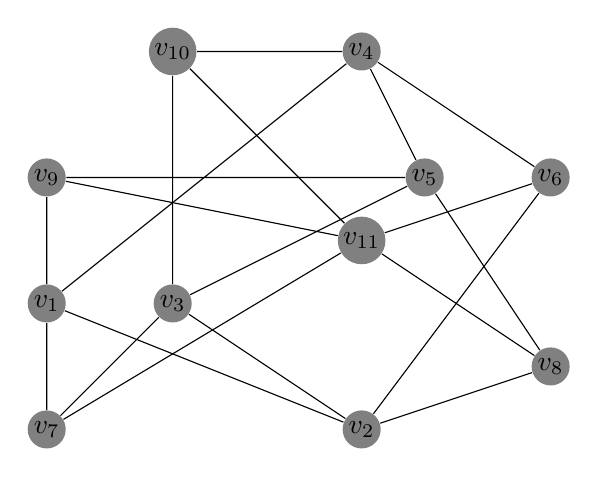
\begin{tikzpicture}[scale=0.8]
\node[circle,fill=gray,inner sep=1pt,minimum size=1mm] (v1) at (0,0) {$v_1$};
\node[circle,fill=gray,inner sep=1pt,minimum size=1mm] (v2) at (5,-2) {$v_2$};
\node[circle,fill=gray,inner sep=1pt,minimum size=1mm] (v3) at (2,0) {$v_3$};
\node[circle,fill=gray,inner sep=1pt,minimum size=1mm] (v4) at (5,4) {$v_4$};
\node[circle,fill=gray,inner sep=1pt,minimum size=1mm] (v5) at (6,2) {$v_5$};
\node[circle,fill=gray,inner sep=1pt,minimum size=1mm] (v6) at (8,2) {$v_6$};
\node[circle,fill=gray,inner sep=1pt,minimum size=1mm] (v7) at (0,-2) {$v_7$};
\node[circle,fill=gray,inner sep=1pt,minimum size=1mm] (v8) at (8,-1) {$v_8$};
\node[circle,fill=gray,inner sep=1pt,minimum size=1mm] (v9) at (0,2) {$v_9$};
\node[circle,fill=gray,inner sep=1pt,minimum size=1mm] (v10) at (2,4) {$v_{10}$};
\node[circle,fill=gray,inner sep=1pt,minimum size=1mm] (v11) at (5,1) {$v_{11}$};


\draw (v4)--(v1)--(v2)--(v3)--(v5)--(v9)--(v1);
\draw (v1)--(v7)--(v3)--(v10)--(v4)--(v6)--(v2)--(v8)--(v11);
\draw (v7)--(v11)--(v10);
\draw (v9)--(v11)--(v6);
\draw (v4)--(v5)--(v8);
\end{tikzpicture}
\end{center}


\end{frame}
\begin{frame}{Step 1}

Exact minimum vertex cover: $X = \{v_1 , v_2 , v_3 , v_4 , v_5 , v_{11}\}$ vs. $2$-approximate: $Y = \{v_1 , v_2 , v_3 , v_4 , v_5 , v_6 , v_8 , v_9 , v_{10} , v_{11}\}$.

\begin{center}
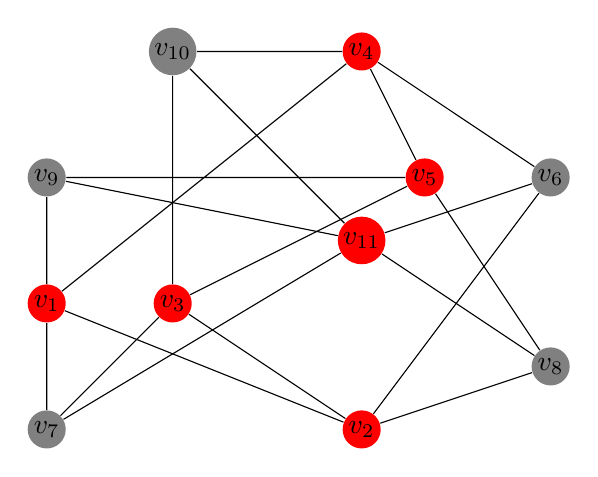
\begin{tikzpicture}[scale=0.8]
\node[circle,fill=red,inner sep=1pt,minimum size=1mm] (v1) at (0,0) {$v_1$};
\node[circle,fill=red,inner sep=1pt,minimum size=1mm] (v2) at (5,-2) {$v_2$};
\node[circle,fill=red,inner sep=1pt,minimum size=1mm] (v3) at (2,0) {$v_3$};
\node[circle,fill=red,inner sep=1pt,minimum size=1mm] (v4) at (5,4) {$v_4$};
\node[circle,fill=red,inner sep=1pt,minimum size=1mm] (v5) at (6,2) {$v_5$};
\node[circle,fill=gray,inner sep=1pt,minimum size=1mm] (v6) at (8,2) {$v_6$};
\node[circle,fill=gray,inner sep=1pt,minimum size=1mm] (v7) at (0,-2) {$v_7$};
\node[circle,fill=gray,inner sep=1pt,minimum size=1mm] (v8) at (8,-1) {$v_8$};
\node[circle,fill=gray,inner sep=1pt,minimum size=1mm] (v9) at (0,2) {$v_9$};
\node[circle,fill=gray,inner sep=1pt,minimum size=1mm] (v10) at (2,4) {$v_{10}$};
\node[circle,fill=red,inner sep=1pt,minimum size=1mm] (v11) at (5,1) {$v_{11}$};


\draw (v4)--(v1)--(v2)--(v3)--(v5)--(v9)--(v1);
\draw (v1)--(v7)--(v3)--(v10)--(v4)--(v6)--(v2)--(v8)--(v11);
\draw (v7)--(v11)--(v10);
\draw (v9)--(v11)--(v6);
\draw (v4)--(v5)--(v8);
\end{tikzpicture}
\end{center}

\end{frame}


\begin{frame}{Steps 2 and 3}
Outside vertices: $\{v_6, v_7, v_8, v_9, v_{10}\}$


For $q = 4$ and the vertex cover $X$, 
\begin{itemize}

\item $v_6$ has no $4$ neighbors in $X$.

\item $v_7$, $v_8$, $v_9$ and $v_{10}$ have no $4$ neighbors in $X$, either. 
\end{itemize}
\begin{center}
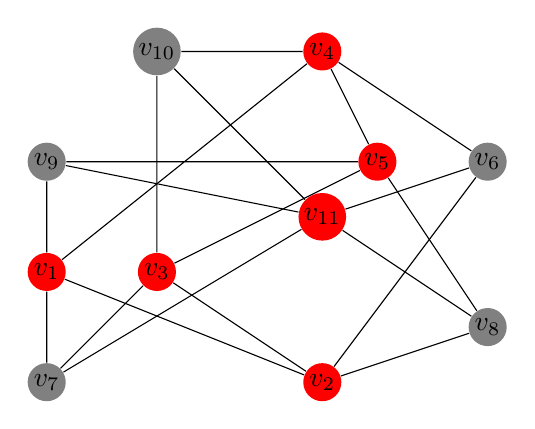
\begin{tikzpicture}[scale=0.7]
\node[circle,fill=red,inner sep=1pt,minimum size=1mm] (v1) at (0,0) {$v_1$};
\node[circle,fill=red,inner sep=1pt,minimum size=1mm] (v2) at (5,-2) {$v_2$};
\node[circle,fill=red,inner sep=1pt,minimum size=1mm] (v3) at (2,0) {$v_3$};
\node[circle,fill=red,inner sep=1pt,minimum size=1mm] (v4) at (5,4) {$v_4$};
\node[circle,fill=red,inner sep=1pt,minimum size=1mm] (v5) at (6,2) {$v_5$};
\node[circle,fill=gray,inner sep=1pt,minimum size=1mm] (v6) at (8,2) {$v_6$};
\node[circle,fill=gray,inner sep=1pt,minimum size=1mm] (v7) at (0,-2) {$v_7$};
\node[circle,fill=gray,inner sep=1pt,minimum size=1mm] (v8) at (8,-1) {$v_8$};
\node[circle,fill=gray,inner sep=1pt,minimum size=1mm] (v9) at (0,2) {$v_9$};
\node[circle,fill=gray,inner sep=1pt,minimum size=1mm] (v10) at (2,4) {$v_{10}$};
\node[circle,fill=red,inner sep=1pt,minimum size=1mm] (v11) at (5,1) {$v_{11}$};


\draw (v4)--(v1)--(v2)--(v3)--(v5)--(v9)--(v1);
\draw (v1)--(v7)--(v3)--(v10)--(v4)--(v6)--(v2)--(v8)--(v11);
\draw (v7)--(v11)--(v10);
\draw (v9)--(v11)--(v6);
\draw (v4)--(v5)--(v8);
\end{tikzpicture}
\end{center}
\end{frame}

\begin{frame}{Step 4}
All of the vertices out of $X$ are unmarked and will be removed. Then the output(kernel) is the set
$\{v_1 , v_2 , v_3 , v_4 , v_5 , v_{11}\}$:


\vspace{1cm}

\begin{center}
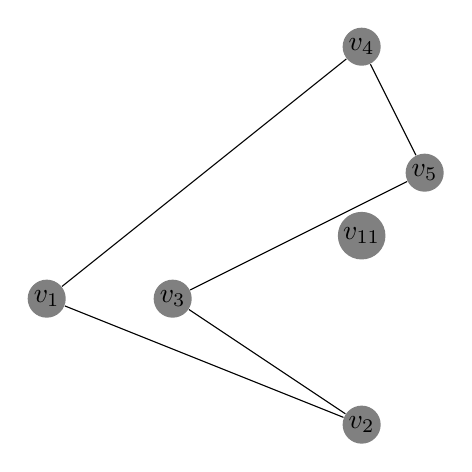
\begin{tikzpicture}[scale=0.8]
\node[circle,fill=gray,inner sep=1pt,minimum size=1mm] (v1) at (0,0) {$v_1$};
\node[circle,fill=gray,inner sep=1pt,minimum size=1mm] (v2) at (5,-2) {$v_2$};
\node[circle,fill=gray,inner sep=1pt,minimum size=1mm] (v3) at (2,0) {$v_3$};
\node[circle,fill=gray,inner sep=1pt,minimum size=1mm] (v4) at (5,4) {$v_4$};
\node[circle,fill=gray,inner sep=1pt,minimum size=1mm] (v5) at (6,2) {$v_5$};
\node[circle,fill=gray,inner sep=1pt,minimum size=1mm] (v11) at (5,1) {$v_{11}$};


\draw (v4)--(v1)--(v2)--(v3)--(v5);
\draw (v4)--(v5);
\end{tikzpicture}
\end{center}
\end{frame}

\begin{frame}{Coloring}

This kernel can be colored with $3$ and therefore with $4$ colors.

\begin{center}
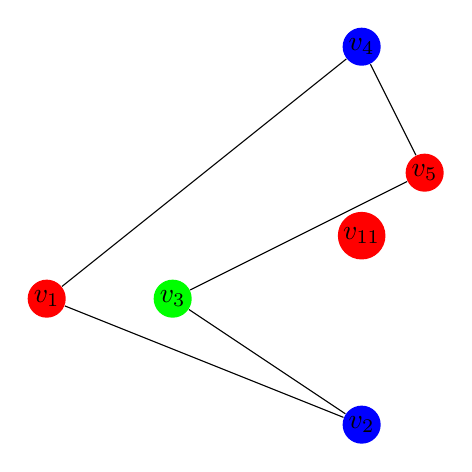
\begin{tikzpicture}[scale=0.8]
\node[circle,fill=red,inner sep=1pt,minimum size=1mm] (v1) at (0,0) {$v_1$};
\node[circle,fill=blue,inner sep=1pt,minimum size=1mm] (v2) at (5,-2) {$v_2$};
\node[circle,fill=green,inner sep=1pt,minimum size=1mm] (v3) at (2,0) {$v_3$};
\node[circle,fill=blue,inner sep=1pt,minimum size=1mm] (v4) at (5,4) {$v_4$};
\node[circle,fill=red,inner sep=1pt,minimum size=1mm] (v5) at (6,2) {$v_5$};
\node[circle,fill=red,inner sep=1pt,minimum size=1mm] (v11) at (5,1) {$v_{11}$};


\draw (v4)--(v1)--(v2)--(v3)--(v5);
\draw (v4)--(v5);
\end{tikzpicture}
\end{center}

\end{frame}
\begin{frame}{Another Steps 3 and 4}
For $q = 3$, and the vertex cover $X$, mark these vertices: $\{v_6, v_7, v_8, v_9, v_{10}\}$:
\begin{wrapfigure}{l}{4cm}
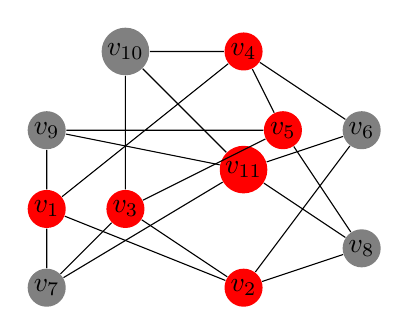
\begin{tikzpicture}[scale=0.5]
\node[circle,fill=red,inner sep=1pt,minimum size=1mm] (v1) at (0,0) {$v_1$};
\node[circle,fill=red,inner sep=1pt,minimum size=1mm] (v2) at (5,-2) {$v_2$};
\node[circle,fill=red,inner sep=1pt,minimum size=1mm] (v3) at (2,0) {$v_3$};
\node[circle,fill=red,inner sep=1pt,minimum size=1mm] (v4) at (5,4) {$v_4$};
\node[circle,fill=red,inner sep=1pt,minimum size=1mm] (v5) at (6,2) {$v_5$};
\node[circle,fill=gray,inner sep=1pt,minimum size=1mm] (v6) at (8,2) {$v_6$};
\node[circle,fill=gray,inner sep=1pt,minimum size=1mm] (v7) at (0,-2) {$v_7$};
\node[circle,fill=gray,inner sep=1pt,minimum size=1mm] (v8) at (8,-1) {$v_8$};
\node[circle,fill=gray,inner sep=1pt,minimum size=1mm] (v9) at (0,2) {$v_9$};
\node[circle,fill=gray,inner sep=1pt,minimum size=1mm] (v10) at (2,4) {$v_{10}$};
\node[circle,fill=red,inner sep=1pt,minimum size=1mm] (v11) at (5,1) {$v_{11}$};


\draw (v4)--(v1)--(v2)--(v3)--(v5)--(v9)--(v1);
\draw (v1)--(v7)--(v3)--(v10)--(v4)--(v6)--(v2)--(v8)--(v11);
\draw (v7)--(v11)--(v10);
\draw (v9)--(v11)--(v6);
\draw (v4)--(v5)--(v8);
\end{tikzpicture}

\end{wrapfigure}

\begin{itemize}
\item $v_6$ has neighbors: $\{v_4 , v_2 , v_{11}\}$

\item $v_7$ has neighbors: $\{v_1 , v_3 , v_{11}\}$

\item $v_8$ has neighbors: $\{v_2 , v_5 , v_{11}\}$ 

\item $v_9$ has neighbors: $\{v_1 , v_5 , v_{11}\}$

\item $v_{10}$ has neighbors: $\{v_4 , v_3 , v_{11}\}$ 
\end{itemize}
\end{frame}

\begin{frame}{$k$-COLORING}
\begin{theorem}
$k$-COLORING for $k \geq 3$ is $NP$-complete.
\end{theorem}

To prove this theorem, it is enough to prove it for $k = 3$.

\begin{itemize}
\item $3$-COLORING is in $NP$ class
\item It is $NP$-hard. 
\end{itemize}


For prove of $NP$-hardness, a reduction from $3$-SAT is used. In order to do the reduction, we need to construct a graph $G_\varphi$ correspondence to a $3$-CNF formula $\varphi$ with $n$ literals $t_1, t_2,\dots, t_n$ and $m$ clauses $C_1, C_2, \dots, C_m$. We should prove $G_\varphi$ is $3$-colorable iff $\varphi$ is satisfiable. 

\end{frame}

\begin{frame}{Proof}
\begin{center}
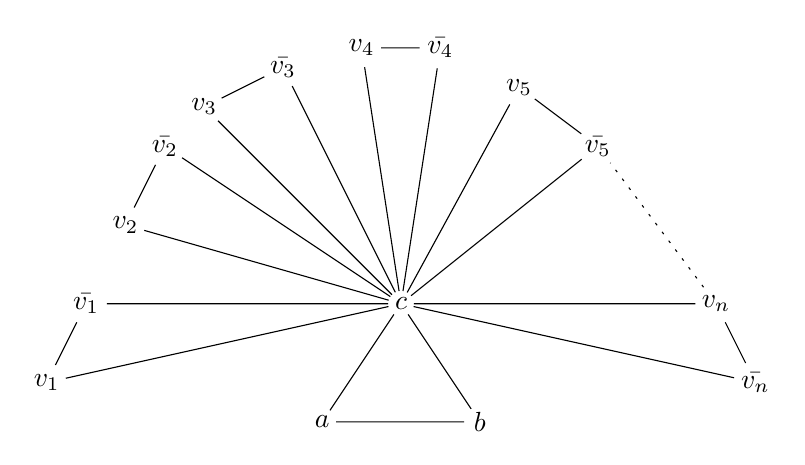
\begin{tikzpicture}
\node[circle,inner sep=1pt,minimum size=1mm] (v1) at (-4,-2.5) {$v_1$};
\node[circle,inner sep=1pt,minimum size=1mm] (nv1) at (-3.5, -1.5) {$\bar{v_1}$};
\node[circle,inner sep=1pt,minimum size=1mm] (v2) at (-3,-0.5) {$v_2$};
\node[circle,inner sep=1pt,minimum size=1mm] (nv2) at (-2.5, 0.5) {$\bar{v_2}$};
\node[circle,inner sep=1pt,minimum size=1mm] (v3) at (-2,1) {$v_3$};
\node[circle,inner sep=1pt,minimum size=1mm] (nv3) at (-1, 1.5) {$\bar{v_3}$};
\node[circle,inner sep=1pt,minimum size=1mm] (v4) at (0,1.75) {$v_4$};
\node[circle,inner sep=1pt,minimum size=1mm] (nv4) at (1, 1.75) {$\bar{v_4}$};
\node[circle,inner sep=1pt,minimum size=1mm] (v5) at (2,1.25) {$v_5$};
\node[circle,inner sep=1pt,minimum size=1mm] (nv5) at (3, 0.5) {$\bar{v_5}$};
\node[circle,inner sep=1pt,minimum size=1mm] (vn) at (4.5,-1.5) {$v_n$};
\node[circle,inner sep=1pt,minimum size=1mm] (nvn) at (5, -2.5) {$\bar{v_n}$};
\node[circle,inner sep=1pt,minimum size=1mm] (c) at (0.5, -1.5) {$c$};
\node[circle,inner sep=1pt,minimum size=1mm] (a) at (-0.5, -3) {$a$};
\node[circle,inner sep=1pt,minimum size=1mm] (b) at (1.5, -3) {$b$};

\draw (c)--(v1)--(nv1)--(c);
\draw (c)--(v2)--(nv2)--(c);
\draw (c)--(v3)--(nv3)--(c);
\draw (c)--(v4)--(nv4)--(c);
\draw (c)--(v5)--(nv5)--(c);
\draw (c)--(vn)--(nvn)--(c);
\draw (c)--(a)--(b)--(c);

\draw [dash pattern={on 1pt off 3pt}](vn) --(nv5);
\end{tikzpicture}
\end{center}
\vspace{1cm}
\end{frame}

\begin{frame}{Proof-continue}
We construct a small OR-gadget graph for each clause $Cj = (x \lor y\lor z)$ in $\varphi$:

\begin{center}
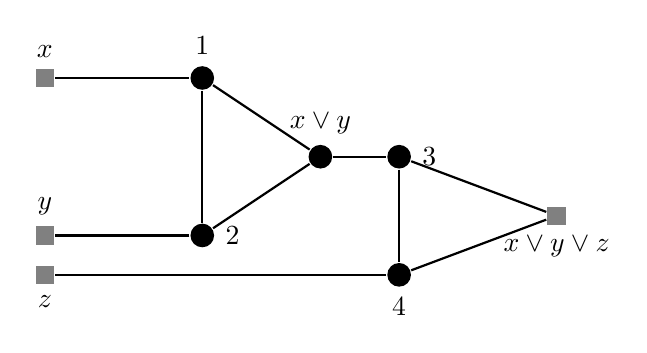
\begin{tikzpicture}[
       thick,
       acteur/.style={
         circle,
         fill=black,
         thick,
         inner sep=2pt,
         minimum size=0.2cm
       }
     ] 
\node[label=$x$,fill=gray] (x) at (-4.5,2.5) {};
\node[label=$y$,fill=gray] (y) at (-4.5, 0.5) {};
\node[label=below:$z$,fill=gray] (z) at (-4.5,0) {};
\node[label=above:1,circle,fill=black,inner sep=1pt,minimum size=3mm] (1) at (-2.5, 2.5) {};
\node[label=right:2,circle,fill=black,inner sep=1pt,minimum size=3mm] (2) at (-2.5,0.5) {};
\node[label=$x\lor y$,circle,fill=black,inner sep=1pt,minimum size=3mm] (xy) at (-1, 1.5) {};
\node[label=right:3,circle,fill=black,inner sep=1pt,minimum size=3mm] (3) at (0,1.5) {};
\node[label=below:4,circle,fill=black,inner sep=1pt,minimum size=3mm] (4) at (0, 0) {};
\node[label=below:$x\lor y\lor z$,fill=gray] (xyz) at (2,0.75) {};

\draw (x)--(1)--(2)--(y);
\draw (1)--(xy)--(2);
\draw (xy)--(3)--(4)--(z);
\draw (3)--(xyz)--(4);

\end{tikzpicture}
\end{center}
\end{frame}


\begin{frame}{Proof-continue}
Now, for each clause $C_j$, we connect its correspondence OR-Gadget to vertex $F$ and $N$ from the triangle.
\begin{center}
\begin{tikzpicture}[scale=0.7]

%\begin{element}[place at cordinate (0,4), scale=1]
%\begin{tikzpicture}[scale=1, every node/.style={scale=1}]
\node[circle,inner sep=1pt,minimum size=1mm] (v1) at (-4,-2.5) {$v_1$};
\node[circle,inner sep=1pt,minimum size=1mm] (nv1) at (-3.5, -1.5) {$\bar{v_1}$};
\node[circle,inner sep=1pt,minimum size=1mm] (v2) at (-3,-0.5) {$v_2$};
\node[circle,inner sep=1pt,minimum size=1mm] (nv2) at (-2.5, 0.5) {$\bar{v_2}$};
\node[circle,inner sep=1pt,minimum size=1mm] (v3) at (-2,1) {$v_3$};
\node[circle,inner sep=1pt,minimum size=1mm] (nv3) at (-1, 1.5) {$\bar{v_3}$};
\node[circle,inner sep=1pt,minimum size=1mm] (v4) at (0,1.75) {$v_4$};
\node[circle,inner sep=1pt,minimum size=1mm] (nv4) at (1, 1.75) {$\bar{v_4}$};
\node[circle,inner sep=1pt,minimum size=1mm] (v5) at (2,1.25) {$v_5$};
\node[circle,inner sep=1pt,minimum size=1mm] (nv5) at (3, 0.5) {$\bar{v_5}$};
\node[circle,inner sep=1pt,minimum size=1mm] (vn) at (4.5,-1.5) {$v_n$};
\node[circle,inner sep=1pt,minimum size=1mm] (nvn) at (5, -2.5) {$\bar{v_n}$};
\node[circle,inner sep=1pt,minimum size=1mm] (n) at (0.5, -1.5) {$N$};
\node[circle,inner sep=1pt,minimum size=1mm] (t) at (-0.5, -3) {$T$};
\node[circle,inner sep=1pt,minimum size=1mm] (f) at (1.5, -3) {$F$};

\draw (n)--(v1)--(nv1)--(n);
\draw (n)--(v2)--(nv2)--(n);
\draw (n)--(v3)--(nv3)--(n);
\draw (n)--(v4)--(nv4)--(n);
\draw (n)--(v5)--(nv5)--(n);
\draw (n)--(vn)--(nvn)--(n);
\draw (n)--(t)--(f)--(n);


\draw [dash pattern={on 1pt off 3pt}](vn) --(nv5);

\begin{scope}[shift={(1.5,-5.5)},rotate=90,scale=0.5, every node/.style={scale=0.5}]

[
       thick,
       acteur/.style={
         circle,
         fill=black,
         thick,
         inner sep=2pt,
         minimum size=0.2cm
       }
     ] 
\node[label=$x_3$,fill=gray] (x) at (-4.5,-7.5) {};
\node[label=$y_3$,fill=gray] (y) at (-4.5, -9.5) {};
\node[label=below:$z_3$,fill=gray] (z) at (-4.5,-10) {};
\node[label=above:1,circle,fill=black,inner sep=1pt,minimum size=3mm] (1) at (-2.5, -7.5) {};
\node[label=right:2,circle,fill=black,inner sep=1pt,minimum size=3mm] (2) at (-2.5,-9.5) {};
\node[label=left:$x_3\lor y_3$,circle,fill=black,inner sep=1pt,minimum size=3mm] (xy) at (-1, -8.5) {};
\node[label=right:3,circle,fill=black,inner sep=1pt,minimum size=3mm] (3) at (0,-8.5) {};
\node[label=below:4,circle,fill=black,inner sep=1pt,minimum size=3mm] (4) at (0, -10) {};
\node[label=right:$x_3\lor y_3\lor z_3$,fill=gray] (xyz1) at (2,-8.75) {};

\draw (x)--(1)--(2)--(y);
\draw (1)--(xy)--(2);
\draw (xy)--(3)--(4)--(z);
\draw (3)--(xyz1)--(4);
\draw [red] (f)--(xyz1)--(n);
   
   
[
       thick,
       acteur/.style={
         circle,
         fill=black,
         thick,
         inner sep=2pt,
         minimum size=0.2cm
       }
     ] 
\node[label=$x_2$,fill=gray] (x) at (-4.5,2.5) {};
\node[label=$y_2$,fill=gray] (y) at (-4.5, 0.5) {};
\node[label=below:$z_2$,fill=gray] (z) at (-4.5,0) {};
\node[label=above:1,circle,fill=black,inner sep=1pt,minimum size=3mm] (1) at (-2.5, 2.5) {};
\node[label=right:2,circle,fill=black,inner sep=1pt,minimum size=3mm] (2) at (-2.5,0.5) {};
\node[label=left:$x_2\lor y_2$,circle,fill=black,inner sep=1pt,minimum size=3mm] (xy) at (-1, 1.5) {};
\node[label=right:3,circle,fill=black,inner sep=1pt,minimum size=3mm] (3) at (0,1.5) {};
\node[label=below:4,circle,fill=black,inner sep=1pt,minimum size=3mm] (4) at (0, 0) {};
\node[label=right:$x_2\lor y_2\lor z_2$,fill=gray] (xyz2) at (2,0.75) {};

\draw (x)--(1)--(2)--(y);
\draw (1)--(xy)--(2);
\draw (xy)--(3)--(4)--(z);
\draw (3)--(xyz2)--(4);  
\draw [red](f)--(xyz2)--(n);

[
       thick,
       acteur/.style={
         circle,
         fill=black,
         thick,
         inner sep=2pt,
         minimum size=0.2cm
       }
     ] 
\node[label=$x_1$,fill=gray] (x) at (-4.5,12.5) {};
\node[label=$y_1$,fill=gray] (y) at (-4.5, 10.5) {};
\node[label=below:$z_1$,fill=gray] (z) at (-4.5,10) {};
\node[label=above:1,circle,fill=black,inner sep=1pt,minimum size=3mm] (1) at (-2.5, 12.5) {};
\node[label=right:2,circle,fill=black,inner sep=1pt,minimum size=3mm] (2) at (-2.5,10.5) {};
\node[label=left:$x_1\lor y_1$,circle,fill=black,inner sep=1pt,minimum size=3mm] (xy) at (-1, 11.5) {};
\node[label=right:3,circle,fill=black,inner sep=1pt,minimum size=3mm] (3) at (0,11.5) {};
\node[label=below:4,circle,fill=black,inner sep=1pt,minimum size=3mm] (4) at (0,10) {};
\node[label=right:$x_1\lor y_1\lor z_1$,fill=gray] (xyz3) at (2,10.75) {};

\draw (x)--(1)--(2)--(y);
\draw (1)--(xy)--(2);
\draw (xy)--(3)--(4)--(z);
\draw (3)--(xyz3)--(4); 
\draw [red](f)--(xyz3)--(n); 
\end{scope}
\draw [dash pattern={on 1pt off 4pt}] (7,-6.5)--(9,-6.5)
\end{tikzpicture}
\end{center}
\end{frame}

\begin{frame}{Proof-continue}
\begin{itemize}
\item $\varphi$ is satisfiable implies $G_\varphi$ is $3$-colorable:

\item $G_\varphi$ is $3$-colorable implies $\varphi$ is satisfiable.
\end{itemize}
\end{frame}

\begin{frame}{DSATUR}
\begin{itemize}

\item DSATUR is a graph coloring algorithm created by Daniel Br\'elaz in 1979. 

\item The run time for the heuristic algorithm DSATUR could be $\mathcal{O}(m \log n)$, for a graph with $n$ vertices and $m$ edges.
\end{itemize}
\begin{definition}
Let $G$ be a simple and partially colored graph. The saturation degree of a vertex is the number of different colors to which it is adjacent (colored vertices).
\end{definition}
\end{frame}

\begin{frame}{DSATUR-Algorithm}

\begin{algorithm}[H]
\begin{algorithmic}[1]
\SetAlgoLined
\DontPrintSemicolon
  \caption{DSATUR (so called because it uses saturation degree)}

\STATE Arrange the vertices by decreasing order of degrees.\\
\STATE Color a vertex of maximal degree with color $1$.\\
\STATE Choose a vertex with a maximal saturation degree. If there is an
\STATE  equality, break the tie by choosing any vertex of maximal degree in the uncolored
subgraph.\\
\STATE Color the chosen vertex with the least possible (lowest numbered)
color.\\
\STATE If all the vertices are colored, stop. Otherwise, return to step 3.\\
\end{algorithmic}
\end{algorithm}
\end{frame}

\begin{frame}{Randall-Brown's Modified Algorithm}
%\newgeometry{left=1in,right=1.2in,top=1in,bottom=1in}
\begin{enumerate}


 
{\tiny  \item Find a maximal clique $K$. Let dimension of clique is $w$. By using DSATUR
beginning with this clique, find an initial coloration with $r$ colors (an
upper bound) and a rank (coloration) order of the vertices. If $w = r$ , stop.\\

\item  Color the vertices of the clique $K$ with $1, 2, . . . w$ successively. For each
vertex $v$ in $G$ let $U(v) \in \{1, 2, . . . r + 1\}$ is the set of colors which can color
$v$. For each vertex $x_k$ out of the clique, let $U(x_k) = U(x_k) - j$ where $j$ is
the color of a vertex in $K$ which is adjacent to $x_k$.\\

\item  Let $k = w + 1$ and $q = r$.\newline
$U(x_k)$ is upper-limited by color $q - 1$ and each vertex is limited by the color
with the same cardinality as its rank). Color $x_k$ with the least possible
color and remove this color from $U(x_k)$ and the color list of all vertices
which are adjacent to $x_k$ , until there is a modification of the $x_k$ color.

\item Let $k = k + 1$ and determine $U(x_k)$.\\

\item  If $U(x_k) = \infty$ go to step 10. Otherwise let $i$ be the least color of $U(x_k)$ and
color $x_k$ with $i$ and $U(x_k) = U(x_k) - i$ then remove this color from the
color set of all vertices adjacent to $x_k$ (with greater rank) until there is a
modification of $x_k$ color. If $i \geq q$ go to step 8.\\

\item  If $k = n$ , let $q = L$ where $L$ is the number of colors used for this coloration
and go to step 7, otherwise go to step 4.\\

\item  If $q = w$, stop. Otherwise , let $x_j$ be the $q$-colored vertex with minimal
rank. If the rank of $x_j$ is equal to $w + 1$ , stop, otherwise let $k = j - 1$ and
go to step 5.\\

\item  If $k = w + 1$ stop. Otherwise, label all unlabeled vertices which have the
following properties:
\begin{enumerate}[(i)]
{\tiny \item with rank $< k$,

\item adjacent to $k$,

\item with none of the colors of vertices of the clique adjacent to $k$ , and
\item with minimal rank among all vertices of their color which are adjacent
to $k$.}
\end{enumerate}
Now let $\nu = k$ . For those vertices are labeled with $k$, if we obtain the rank
$k$ or more in a partial coloration, the label should be removed.\\


\item  Let $k = t$ where $t$ is the maximal rank of labeled vertices, which have rank $< k$. For $k < i \leq \nu$ , $U(x_i)$ is the set of colors defind in step 3. Go to step 5.\\


\item  If none of the colors is possible for $x_k$ (all are tested), then backtracking
should be done. For this go to step 8.\\}
\end{enumerate}

\end{frame}

\begin{frame}{Computational Experiments}
Solve ILP for vertex cover:
\begin{itemize}
\item Make a model with AMPL for vertex cover restricted by maximal cliques.
\item Solving it with CPLEX samples.
\end{itemize}
\end{frame}

\begin{frame}[fragile]{AMPL Model for vertex cover restricted to maximal cliques}


\begin{verbatim}
# Declarations
set V;
set E within V cross V;
set Idx;
set Q within Idx cross V;
set cnt within Idx cross V;
var x {v in V} binary;
# integrality constraints.
# Objective Function
minimize cover_size: sum { v in V } x[v];
# Constraints
subject to clique {c in Idx}:
sum {(a, b) in Q: a=c} x[b] >= card{(a,b) in Q: a=c}-1;
\end{verbatim}

\end{frame}

\begin{frame}{Conclusion}
\begin{itemize}
\item Summary
\item Future Work
\begin{itemize}
\item Which kind of graphs and why
\item probable to identify some indexes in the graph and relate performance of kernelization to them.
\end{itemize}
\end{itemize}

\end{frame}


\end{document}
}
